% Improved Modern Resume Template for Puneet Ludu
% Class and package configuration
\documentclass[11pt,letterpaper]{article}

% Packages
\usepackage[utf8]{inputenc}
\usepackage[T1]{fontenc}
\usepackage{fontawesome5}
\usepackage{geometry}
\usepackage{titlesec}
\usepackage{enumitem}
\usepackage{hyperref}
\usepackage{xcolor}
\usepackage{tabularx}
\usepackage{array}
\usepackage{setspace}
\usepackage{tikz}
\usepackage{tcolorbox}
\usepackage{ragged2e}
\usepackage{pgfplots}
\usepackage{pgf-pie}
\pgfplotsset{compat=1.16}

% Set page margins - UPDATED: reduced margins to use more horizontal space
\geometry{left=0.5in, right=0.5in, top=0.5in, bottom=0.5in}

% Define colors
\definecolor{namecolor}{RGB}{50, 50, 50}
\definecolor{sectioncolor}{RGB}{30, 30, 30}
\definecolor{linkcolor}{RGB}{0, 0, 200}
\definecolor{impactcolor}{RGB}{70, 70, 70}
\definecolor{yearcolor}{RGB}{120, 120, 120}
\definecolor{sectionbg}{RGB}{245, 245, 245}

% Chart colors
\definecolor{chartblue}{RGB}{54, 162, 235}      % Architecture
\definecolor{chartyellow}{RGB}{255, 206, 86}    % MLOps
\definecolor{chartorange}{RGB}{255, 159, 64}    % Leadership
\definecolor{chartgreen}{RGB}{138, 194, 74}     % Prompt Engineering
\definecolor{chartred}{RGB}{255, 99, 132}       % Coding
\definecolor{chartpurple}{RGB}{153, 102, 255}   % Modeling
\definecolor{chartteal}{RGB}{75, 192, 192}      % Data Eng.

% Configure hyperref
\hypersetup{
    colorlinks=true,
    urlcolor=linkcolor,
    pdftitle={Puneet Ludu Resume},
    pdfauthor={Puneet Ludu},
}

% Remove page numbers
\pagenumbering{gobble}

% Set paragraph spacing
\setlength{\parindent}{0pt}
\setlength{\parskip}{3pt}

% Custom font size commands
\newcommand{\normalsizesection}{\normalsize}
\newcommand{\smallersection}{\small}
\newcommand{\smallestsection}{\footnotesize}
\newcommand{\tinyfootnote}{\fontsize{8pt}{9pt}\selectfont} % Changed from 8.5pt to 8pt

% Configure section formatting with colored box
\titleformat{\section}
    {\Large\bfseries\color{sectioncolor}}
    {}
    {0em}
    {}
    
\titlespacing{\section}{0pt}{8pt}{2pt}

% Custom section with background
\newcommand{\sectionbox}[1]{%
    \vspace{0.2em}
    \begin{tcolorbox}[
        colback=sectionbg,
        colframe=sectionbg,
        width=\textwidth,
        left=5pt,
        right=5pt,
        top=2pt,
        bottom=2pt,
        boxrule=0pt,
        arc=0pt,
        boxsep=0pt,
    ]
    \section*{#1}
    \end{tcolorbox}
    \vspace{-0.3em}
}

% Custom commands
\newcommand{\yearsright}[1]{{\footnotesize\bfseries\color{yearcolor} #1}}
\newcommand{\impact}[1]{\textit{Impact: #1}}
\newcommand{\tech}[1]{\textit{(#1)}}
\newcommand{\approach}[1]{[#1]}
\newcommand{\entryspace}{\vspace{-1pt}}

% Custom environment for resume entries with hierarchical structure
\newenvironment{resumeentry}[5]{%
    \noindent\textbf{#1}\if\relax\detokenize{#1}\relax\else, \fi%
    \if\relax\detokenize{#2}\relax\else\textit{#2}, \fi%
    \if\relax\detokenize{#3}\relax\else\textbf{#3}, \fi%
    \if\relax\detokenize{#4}\relax\else#4\fi%
    \if\relax\detokenize{#5}\relax\else\hfill\yearsright{#5}\fi\\[-2pt]
}{\vspace{-1pt}}

% Project entry with indentation and hierarchical structure
\newenvironment{projectentry}{%
    \leftskip=0.5cm
    \par\noindent
}{\par\leftskip=0cm\vspace{-2pt}}

% Project description with deeper indentation
\newenvironment{projectdesc}{%
    \leftskip=1.0cm
    \footnotesize
    \par\noindent
}{\par\leftskip=0cm\smallersection\vspace{-3pt}}

% Link with icon
\newcommand{\iconlink}[3]{%
    #1~\href{#2}{#3}%
}

% Project icon - new command for project icons
\newcommand{\projicon}[1]{%
    {\small\color{gray!70}#1}~%
}

% Begin document
\begin{document}

% Header with side-by-side layout
\begin{minipage}[t]{0.6\textwidth}
    \vspace{0pt}
    \fontsize{24pt}{28pt}\selectfont\textbf{\color{namecolor}Puneet Ludu}\\[8pt]
    \footnotesize puneet.ludu@gmail.com | New York, NY | +1-(716) 867-4344 | \href{https://puneet.io}{puneet.io}
\end{minipage}%
\begin{minipage}[t]{0.4\textwidth}
    \vspace{0pt}
    \raggedright
    \footnotesize\iconlink{\faGithub}{https://github.com/puneetsl}{https://github.com/puneetsl}\\
    \footnotesize\iconlink{\faLinkedin}{https://www.linkedin.com/in/puneetsl}{https://www.linkedin.com/in/puneetsl}\\
    \footnotesize\iconlink{\faDatabase}{https://www.kaggle.com/puneetsl}{https://www.kaggle.com/puneetsl}
\end{minipage}

\vspace{0mm}
\noindent\rule{\textwidth}{0.4pt}
\vspace{-2mm}

% Experience section
\sectionbox{Experience \hfill \normalsize 10+ years}
\smallersection

\begin{resumeentry}{Machine Learning Engineer}{Sep 2021 -- Present}{Zillow (Zestimate)}{Remote}{4Y}
\end{resumeentry}

% Active Listing Comps - Leading with production impact
\begin{projectentry}
    \projicon{\faDatabase} \textbf{Active Listing Comps Engine} \tech{Apache Spark, Metaflow, H3 Geospatial} \approach{Similarity Scoring + Batch/REST APIs}
\end{projectentry}

\begin{projectdesc}
    Architected similar listings comparison engine powering Zillow Showcase's go-to-market strategy. Built scalable batch pipeline and real-time API using geospatial indexing (H3) and customizable ranking algorithms. System processes millions of listings daily, generating business-critical performance metrics.\\[1pt]
    \impact{30\% listing wins, 75\% engagement lift for Showcase - metrics used across sales, marketing, and investor communications}
\end{projectdesc}

% Interactive CMA - with integrated explainability
\begin{projectentry}
    \projicon{\faChartLine} \textbf{Interactive CMA \& Realtime Valuation Platform} \tech{Django, DocumentDB, PyTorch} \approach{Siamese Networks + Explainability}
\end{projectentry}

\begin{projectdesc}
    Architected 0-to-1 platform integrating real-time valuations, property embeddings, and amenity explanations. Designed APIs for comparative analysis and interactive agent reporting. Led technical decisions on ML integration and service architecture. Platform launching soon.\\[1pt]
    \impact{Foundation for new agent revenue products, establishing real-time ML serving patterns}
\end{projectdesc}

% Infrastructure modernization with enhanced Staff-level language
\begin{projectentry}
    \projicon{\faServer} \textbf{Zestimate Infrastructure Modernization} \tech{Terraform, AWS, Kubeflow, Metaflow, Docker}
\end{projectentry}

\begin{projectdesc}
    Drove migration of critical ML pipelines from legacy systems to containerized infrastructure. Established CI/CD patterns, monitoring standards, and deployment practices that reduced operational overhead. Mentored team on modern MLOps practices and infrastructure-as-code principles.\\[1pt]
    \impact{\$500K annual savings, 80\% faster deployments, 95\% reduction in on-call alerts through proactive monitoring}
\end{projectdesc}

% Combining Amenity Adjustment and LLM tools - both in beta/development
\begin{projectentry}
    \projicon{\faBuilding} \textbf{Next-Gen Explainability: Amenity Adjustment \& LLM Tools} \tech{PyTorch, DeepLift, LangChain} 
\end{projectentry}

\begin{projectdesc}
    Developing ML explainability service for dollar-value feature attributions and LLM tools for automated Zestimate queries. Building APIs for property data retrieval, comparative analysis, and natural language explanations. Both initiatives in beta, targeting improved user trust and reduced support burden.\\[1pt]
    \impact{Foundation for automated customer support and transparent valuations}
\end{projectdesc}

% Technical contributions - specific and accurate
\begin{projectentry}
    \projicon{\faCode} \textbf{Engineering Excellence \& Pipeline Stability}
\end{projectentry}

\begin{projectdesc}
    Established MR best practices (stacked MRs, pre-submission checklists) and documentation standards. Led weekly bug bashes targeting low-effort, high-impact improvements. Mentored interns and junior engineers.\\[1pt]
    \impact{Improved Zestimate pipeline success rate from 75\% to 85\%, reducing production incidents}
\end{projectdesc}

\begin{resumeentry}{Machine Learning Engineer}{May 2020 - Sep 2021}{OkCupid (Match.com)}{New York City}{1.5Y}
\end{resumeentry}

\begin{projectentry}
    \projicon{\faSort} \textbf{Discount Optimization} \tech{Python, Keras, TensorFlow, Weights and Biases} \approach{\href{https://blog.research.google/2016/06/wide-deep-learning-better-together-with.html}{Wide\&Deep}}
\end{projectentry}

\begin{projectdesc}
    Led efforts to optimize subscription pricing (discounts) to maximize revenue for OkCupid. Implemented end-to-end ML pipelines, feature engineering, modeling, alerting, etc.\\[1pt]
    \impact{Increased overall revenue by \textbf{6\%} through A/B testing against assigned prices}
\end{projectdesc}

\begin{resumeentry}{Machine Learning Engineer}{Apr 2015 - May 2020}{FactSet}{New York City}{5Y}
\end{resumeentry}

% Combining NLP/ML projects for financial data extraction
\begin{projectentry}
    \projicon{\faMicrophone} \textbf{ML-Powered Financial Data Extraction} \tech{Python, TensorFlow, Keras, Sagemaker} \approach{CNN, ELMo, BiLSTM}
\end{projectentry}

\begin{projectdesc}
    Led multiple ML initiatives: (1) Speaker identification system for earnings calls using spectrograms and CNNs, (2) Private company fact extraction from 1.6M websites using ELMo/BiLSTM. Built end-to-end pipelines from data collection to deployment.\\[1pt]
    \impact{20\% reduction in human-hours for earnings call processing, automated extraction from millions of documents} [\href{https://drive.google.com/file/d/1nF485POZoE2YsYuQHdvUHO1GbwkQUDfL/view}{\faFile}]
\end{projectdesc}

% Combining search-related projects
\begin{projectentry}
    \projicon{\faSearch} \textbf{Financial Document Search \& Ranking Systems} \tech{Apache Spark, Java, Python} \approach{Distributed Trie, N-gram LM, Vector Space}
\end{projectentry}

\begin{projectdesc}
    Architected search infrastructure: (1) Type-ahead and query expansion for document search, (2) Real-time formula ranking using language models, (3) Duplicate document detection service. Scaled to handle thousands of queries/documents per day.\\[1pt]
    \impact{Improved formula ranking from 5.6 to 2.3, 66\% faster document processing, powered StreetAccount trending news}
\end{projectdesc}

\begin{resumeentry}{ML Research Engineer}{July 2011 - July 2013}{\href{https://en.wikipedia.org/wiki/Tata_Research_Development_and_Design_Centre}{Tata Research Development and Design Centre}}{India}{2Y}
\end{resumeentry}

\begin{projectentry}
    \projicon{\faChartLine} \textbf{Event Detection in Time Series} \tech{Java, Python, RapidMiner} \approach{SVM - RBF} \href{http://arxiv.org/pdf/1408.3733v1.pdf}{\faFilePdf}
\end{projectentry}

\begin{projectdesc}
    Wrote an algorithm based on Shape Context for finding frequently occurring patterns and events, with as good results as SAX, DTW etc. with \textbf{7\%} better results in the particular domain of car sensors.
\end{projectdesc}

\begin{projectentry}
    \projicon{\faDatabase} \textbf{\href{https://ieeexplore.ieee.org/abstract/document/6597127}{Data Harmonization Framework (DHF)}} \tech{Java, Apache Pig}
\end{projectentry}

\begin{projectdesc}
    Implemented an ETL framework that exploits the power of map-reduce and big-databases to fuse incongruous enterprise data from disparate sources in near real time.
\end{projectdesc}

\normalsizesection

\vspace{30pt} % Add vertical space to push Skills section to next page

% Skills section
\sectionbox{Skills}
\smallersection

\noindent\textbf{Languages} \hspace{2mm} Python • Java • C/C++ • Bash • Javascript • HTML • SQL

\vspace{1pt}
\noindent\textbf{Frameworks} \hspace{0.5mm} PySpark • FastAPI • Metaflow • KubeFlow • TensorFlow/PyTorch • W\&B • DataBricks  • Django

\vspace{1pt}
\noindent\textbf{AI Dev \& Infra} \hspace{1mm} Cursor • V0 • MongoDB • Pinecone • Docker • Kubernetes • Terraform • Gitlab CI

\vspace{1pt}
\noindent\textbf{Leadership} \hspace{4mm} System Design • Technical Mentoring • Cross-functional Collaboration • Code Reviews • Architecture Decisions

\normalsizesection

% Publications section
\sectionbox{Publications \hfill \normalsize\iconlink{\faGraduationCap}{https://scholar.google.com/citations?user=NrYKcaMAAAAJ\&hl=en}{Google Scholar profile}}
\tinyfootnote % Custom size between footnotesize and scriptsize

\noindent\textbf{\href{http://dl.acm.org/citation.cfm?id=2806657}{Inferring Latent Attributes of an Indian Twitter user using Celebrities and Class Influencers}} \hfill \href{https://www.youtube.com/watch?v=9BtWs3Rn2Ng}{\faYoutube} ACM Hypertext 2015

\vspace{-1pt}
\noindent\textbf{\href{http://arxiv.org/abs/1405.6667}{Inferring gender of a Twitter user using celebrities it follows}} \hfill CORR 2014

\vspace{-1pt}
\noindent\textbf{\href{http://arxiv.org/abs/1206.2484}{Architecture for Automated Tagging and Clustering of Song Files According to Mood}} \hfill IJCSI, 2010

\normalsizesection

% Education section
\sectionbox{Education}
\smallersection

\noindent\textbf{Master of Science} in Computer Science, State University of New York, Buffalo, NY \hfill 2014

\vspace{-1pt}
\noindent\textbf{B. Tech.} in Computer Science and Engineering, JIIT, India \hfill 2010

\normalsizesection

% Personal Projects section
\sectionbox{Personal Projects / Extra Curricular}
\smallersection

\begingroup
\setlength{\tabcolsep}{6pt}
\renewcommand{\arraystretch}{1.0}
\begin{tabularx}{\textwidth}{@{} l X @{}}
\textbf{\iconlink{\faUsers}{https://sites.google.com/view/w-mufin/organizers}{Organizer @ MUFin}} & Committee member, organizer and reviewer to the MUFin Workshop at top conferences, focusing on innovative approaches to modeling uncertainty in the financial sector \textit{(AAAI2023, PKDD2022)} \\[3pt]

\textbf{\iconlink{\faGithub}{https://github.com/puneetsl/lotion}{Lotion}} & Unofficial Notion.so Desktop app for Linux \textit{(2K+ GitHub stars / 60K+ Clones \& Downloads)} \\[3pt]

\textbf{\iconlink{\faGithub}{https://github.com/puneetsl/Romadeva}{Romadeva}} & Tool to convert Roman script to Indic(Devanagari) script \textit{(Used by https://translatorswithoutborders.org)} \\[3pt]

\textbf{\iconlink{\faGithub}{https://github.com/puneetsl/jtextbrew}{jTextBrew}} & A JAVA library for fuzzy string matching, based on TextBrew algorithm by Chris Brew \\[3pt]

\textbf{\iconlink{\faQuestionCircle}{https://www.facebook.com/photo.php?fbid=10153613108040010\&set=a.10153613186550010\&type=3\&theater}{Quena}} & Question and Answering system – Indexed 1.6 Million Wikipedia documents, designed a question parser and a ranking algorithm based on popularity. \textit{(Apache Solr, NER, POS tagger)}
\end{tabularx}
\endgroup

\normalsizesection

% Add a simple skill visualization - Fixed charts section with better spacing
\begin{center}
\sectionbox{Professional Focus \& Evolution}
\end{center}

% Improved spacing between charts and adjusted minipage widths
\begin{minipage}[t]{0.48\textwidth}
\begin{center}
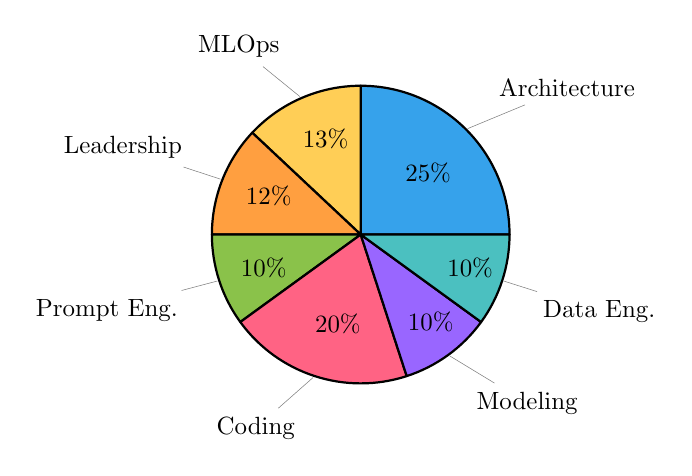
\begin{tikzpicture}[scale=0.9, transform shape]
\pie[
  radius=2.1,
  color={chartblue, chartyellow, chartorange, chartgreen, chartred, chartpurple, chartteal},
  text=pin,
  sum=100,
  after number=\%,
  before number=\phantom{0},
  every pin/.style={align=center},
  every pin label/.style={font=\footnotesize}
]{25/Architecture, 13/MLOps, 12/Leadership, 10/Prompt Eng., 20/Coding, 10/Modeling, 10/Data Eng.}
\end{tikzpicture}
\end{center}
\end{minipage}%
\hfill% Use hfill for better automatic spacing
\begin{minipage}[t]{0.48\textwidth}
\begin{center}
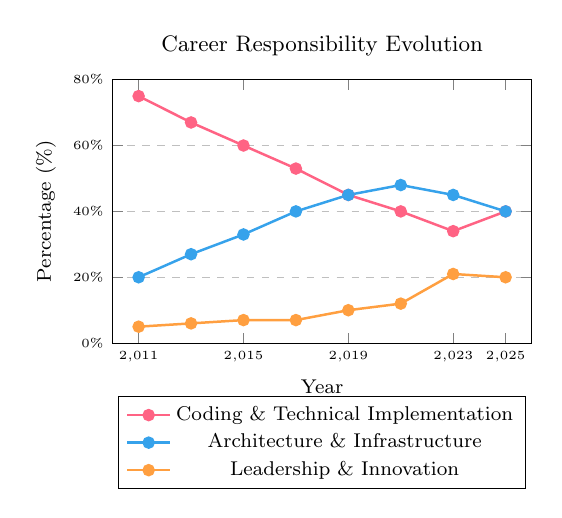
\begin{tikzpicture}[scale=0.9, transform shape]
\begin{axis}[
    width=7.5cm,
    height=5.3cm,
    title={Career Responsibility Evolution},
    xlabel={Year},
    ylabel={Percentage (\%)}, % Added % symbol to the y-axis label
    xmin=2010, xmax=2026,
    ymin=0, ymax=80,
    xtick={2011,2015,2019,2023,2025},
    ytick={0,20,40,60,80},
    yticklabel={\pgfmathprintnumber{\tick}\%}, % Added % symbol to the tick labels
    legend style={at={(0.5,-0.2)}, anchor=north, legend columns=1, font=\footnotesize},
    ymajorgrids=true,
    grid style=dashed,
    tick label style={font=\tiny},
    title style={font=\small},
    label style={font=\footnotesize},
]

\addplot[
    color=chartred,
    mark=*,
    line width=1pt,
    ]
    coordinates {
    (2011,75)(2013,67)(2015,60)(2017,53)(2019,45)(2021,40)(2023,34)(2025,40)
    };
\addlegendentry{Coding \& Technical Implementation}

\addplot[
    color=chartblue,
    mark=*,
    line width=1pt,
    ]
    coordinates {
    (2011,20)(2013,27)(2015,33)(2017,40)(2019,45)(2021,48)(2023,45)(2025,40)
    };
\addlegendentry{Architecture \& Infrastructure}

\addplot[
    color=chartorange,
    mark=*,
    line width=1pt,
    ]
    coordinates {
    (2011,5)(2013,6)(2015,7)(2017,7)(2019,10)(2021,12)(2023,21)(2025,20)
    };
\addlegendentry{Leadership \& Innovation}

\end{axis}
\end{tikzpicture}
\end{center}
\end{minipage}

\end{document}